\section{Architecture Integration}

\subsection{Model Support}

\begin{table}[H]
\centering
\small
\begin{tabular}{lllll}
\toprule
\textbf{Model} & \textbf{Attention path} & \textbf{Nested?} & \textbf{RoPE?} & \textbf{GQA?} \\
\midrule
DistilBERT & \texttt{layer[i].attention} & No & No & No \\
RoBERTa & \texttt{layer[i].attention.self} & Yes & No & No \\
GPT-2 & \texttt{h[i].attn} & No & No & No \\
Qwen3.5 & \texttt{layers[i].self\_attn} & No & Yes & Yes \\
\bottomrule
\end{tabular}
\end{table}

\subsection{Weight Extraction}

UniversalAdapter first, then fallbacks:

\subsubsection{GPT-2 Fused Conv1D}

\begin{lstlisting}
c\_w = src.c\_attn.weight
if c\_w.shape[0] \textless{} c\_w.shape[1]: c\_w = c\_w.t()
q\_w, k\_w, v\_w = c\_w.chunk(3, dim=0)
o\_w = src.c\_proj.weight.t()
\end{lstlisting}

\subsubsection{RoBERTa Nested}

\begin{lstlisting}
s = src.self
q\_w = s.query.weight
k\_w = s.key.weight
v\_w = s.value.weight
o\_w = src.output.dense.weight
\end{lstlisting}

\subsubsection{Flat Modules}

Standard attributes.

\subsection{Soft Fallback}

After UniversalAdapter fails, we log a warning. But the code still 
raises \texttt{RuntimeError} at the end if any required projection is missing -- 
this can kill the module.

\subsection{Landmark Scorer Architecture}

LayerNorm over $3F$ features $\to$ Linear($3F$, 64) $\to$ GELU $\to$ Linear(64, 1).

\subsection{Correction Matrix Shape}

$W_\text{corr} \in \mathbb{R}^{H \times d_h \times d_h}$, initialized 
as $I_{d_h}$ per head.

\textbf{Note.} For $H = 12, d_h = 64$, this is $12 \times 64 \times 64 = 49,152$ 
parameters per layer.

\subsection{Local-Global Gate}

Per-head scalar $g_h \in (0, 1)$, initialized to $\sigma(-2) \approx 0.12$.

\textbf{Note.} The gate is applied \textbf{before} the \texttt{output\_scale} in 
LEKAv1 -- here, there is no \texttt{output\_scale}.

\subsection{Nested Encoder Bypass}

For RoBERTa, \texttt{is\_nested\_encoder = True}. Raw context returned.

\subsection{Causal Masking}

\textbf{Global branch.} Masked via landmark positions:

\begin{lstlisting}
q\_pos = torch.arange(N).view(1, 1, N, 1)
k\_land\_pos = land\_idx.unsqueeze(2)
causal\_land\_mask = (k\_land\_pos \textless{}= q\_pos)
attn\_weights = attn\_weights.masked\_fill(~causal\_land\_mask, -1e4)
\end{lstlisting}

\textbf{Local branch.} Standard causal mask.

\subsection{Injection Algorithm}

\textbf{Algorithm 2:} Inject LEKAv2 into a model
\begin{lstlisting}
Input:  model M, config c
Output: M with attention replaced

1: for layer in transformer\_layers(M):
2:     src $\leftarrow$ extract\_attention(layer)
3:     if src is None or is\_already\_injected: continue
4:     try:
5:         new $\leftarrow$ LEKAv2Attention(c, old\_attn=src)
6:         replace(layer, new)
7:     except Exception:
8:         log\_error; continue
9: return M
\end{lstlisting}

\subsection{Double-Injection Guard}

\begin{lstlisting}
if isinstance(src\_attn, LEKAv2Attention): return None
if "LEKAv2" in src\_attn.\_\_class\_\_.\_\_name\_\_: return None
if "LEKA" in src\_attn.\_\_class\_\_.\_\_name\_\_: return None
\end{lstlisting}

\subsection{Registry}

\begin{lstlisting}
@ATTENTION\_REGISTRY.register("leka\_v2")
@ATTENTION\_REGISTRY.register("leka\_v2\_attention")
class LEKAv2Attention(BaseAttention):
    ...
\end{lstlisting}

\subsection{Cross-Attention}

Not supported.
\begin{lstlisting}

---
\end{lstlisting}

\begin{figure}[H]
\centering
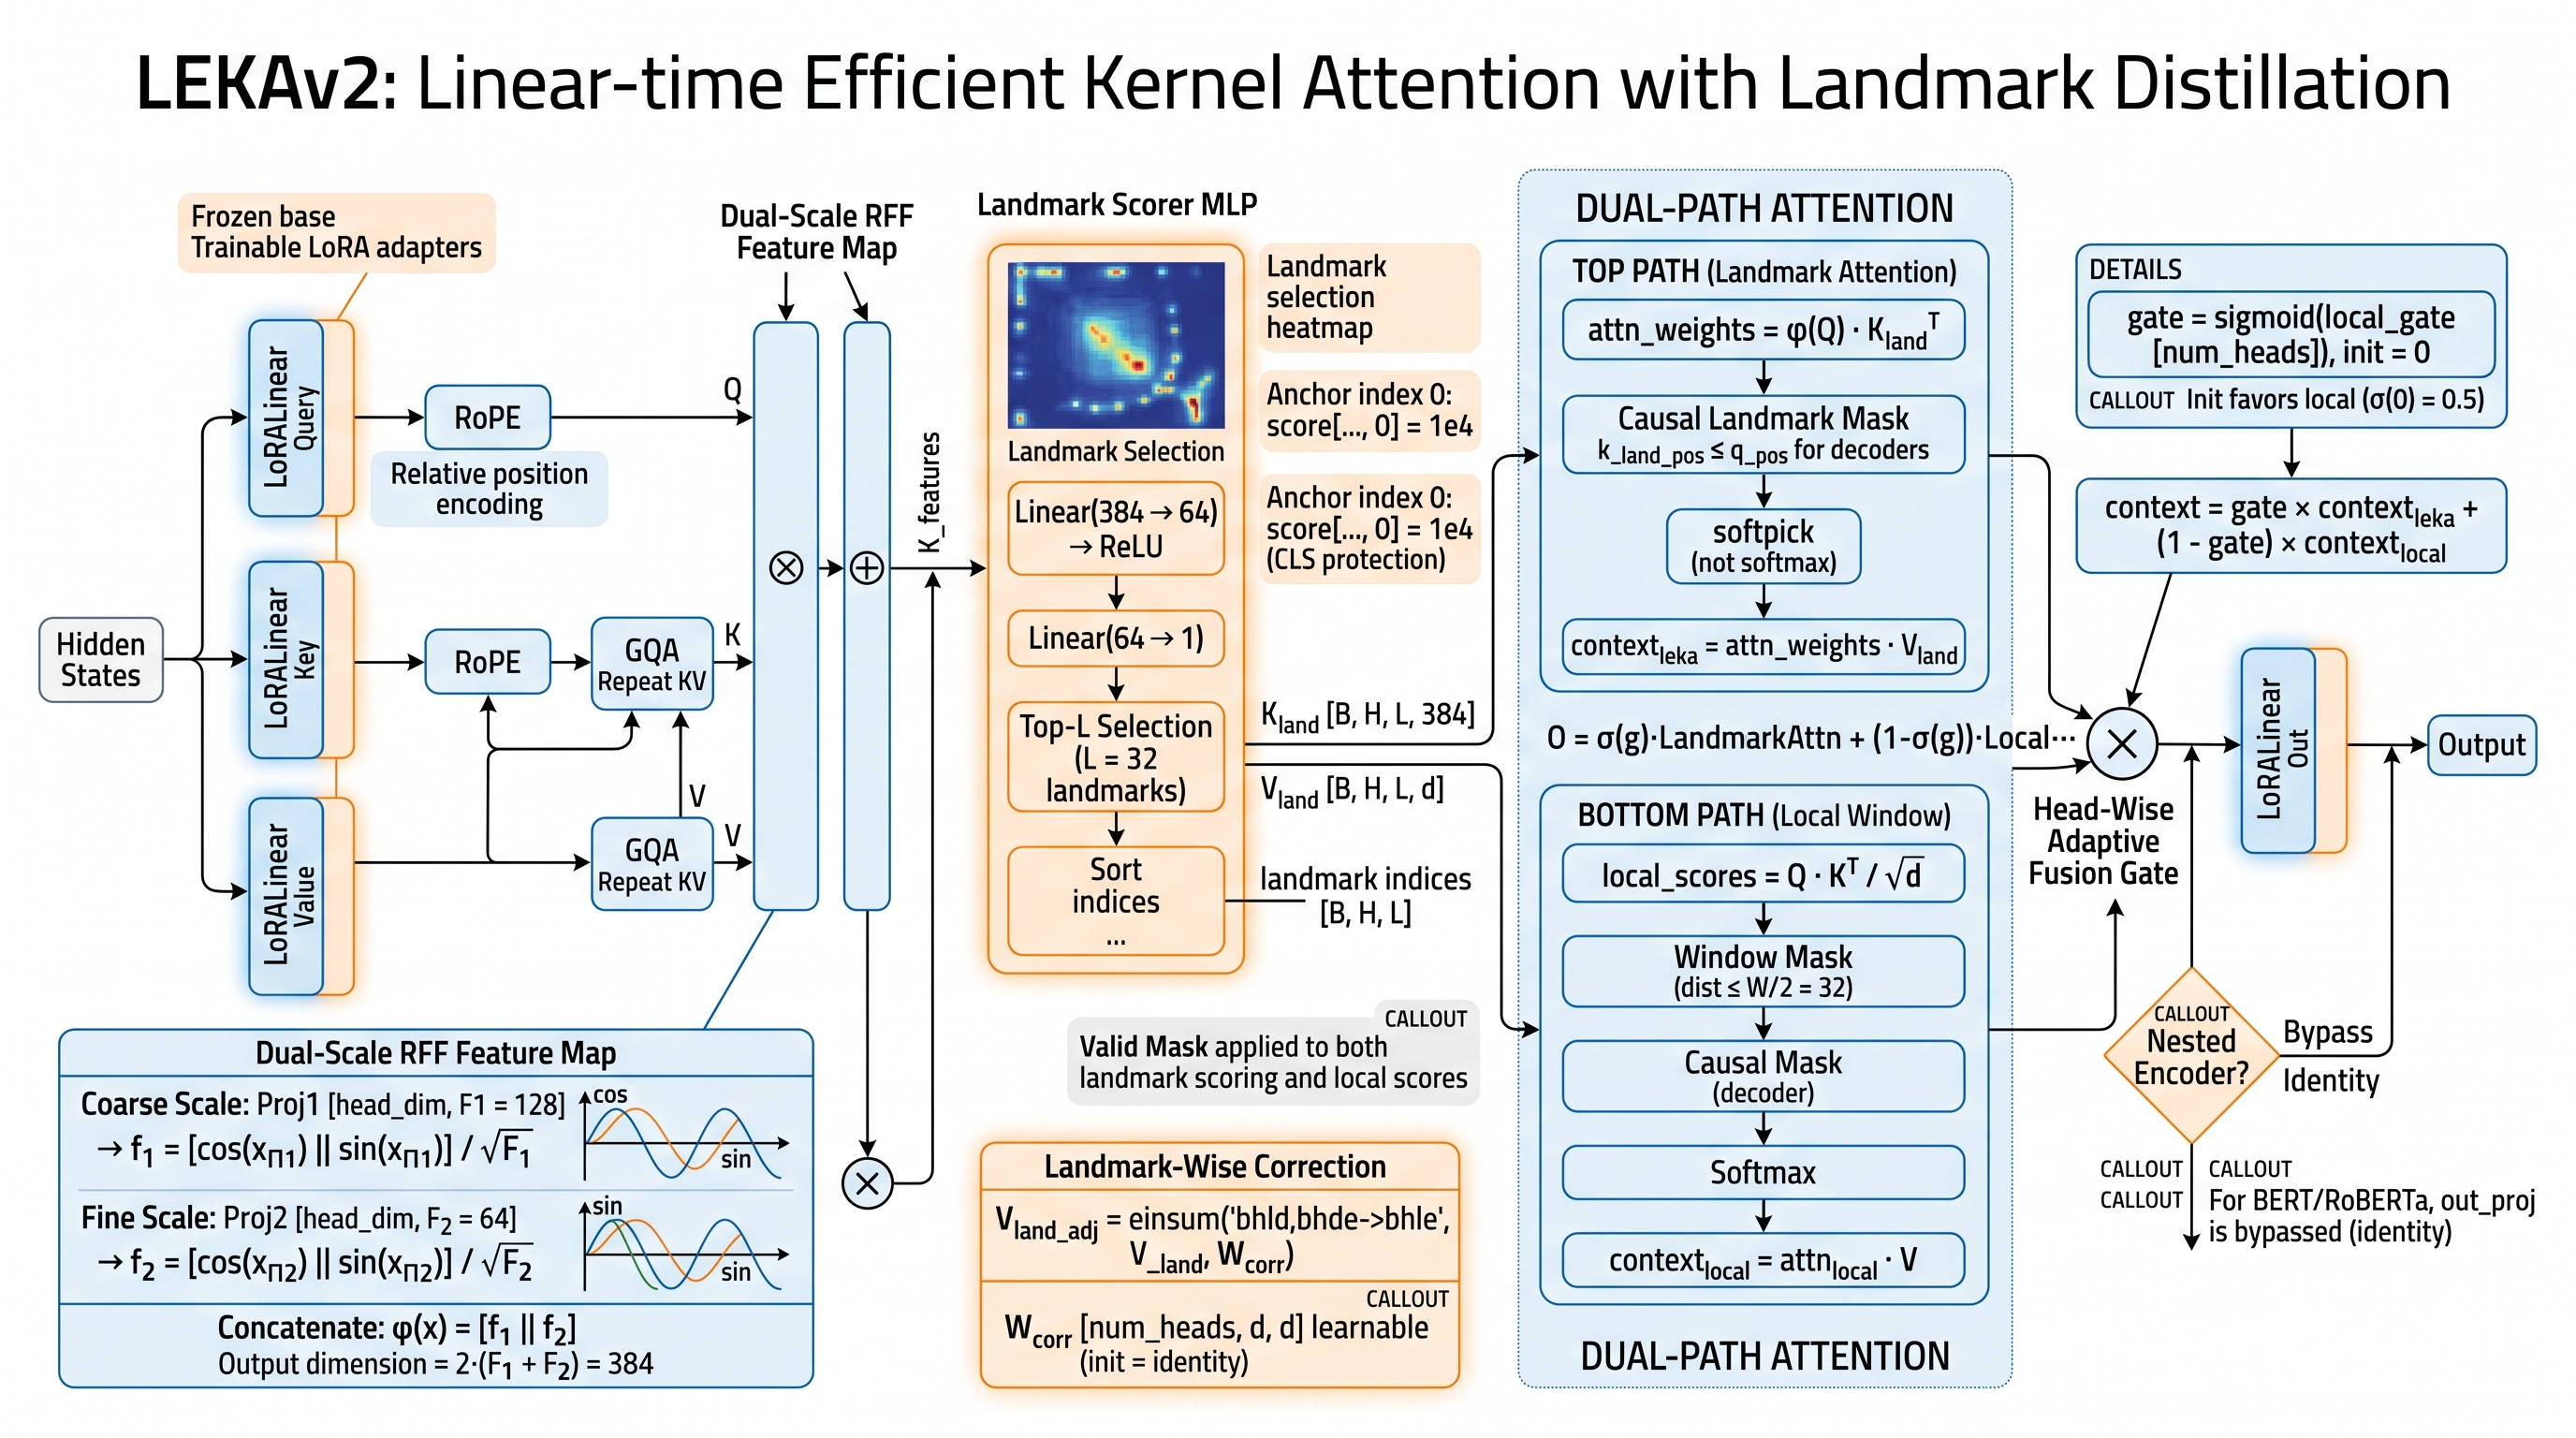
\includegraphics[width=\linewidth]{figures/architecture.jpeg}
\caption{High-level architectural diagram of leka\_v2.}
\label{fig:arch_leka-v2}
\end{figure}

